\documentclass[tikz,border=1mm]{standalone} 
\usepackage{amsfonts,amssymb,amsmath,bm}
\usetikzlibrary{positioning,shadows,shapes.symbols,shapes.geometric}

% colors
\definecolor{myblue}{rgb}{0.4, 0.6, 0.8}
\definecolor{mycoral}{rgb}{0.97,0.51,0.47}
\definecolor{mygreen}{rgb}{0.66,0.89,0.63}
\definecolor{myocra}{rgb}{1, 0.8, 0.4}
\definecolor{mypurple}{rgb}{0.7, 0.6, 0.9}

\begin{document}
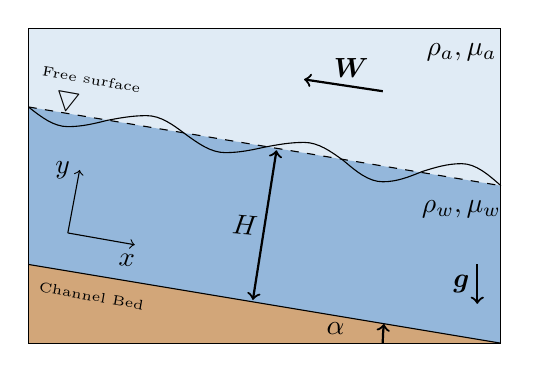
\begin{tikzpicture}

\centering
% filling
\fill [myblue, opacity=0.2] (-3,2) -- (-3,1) -- (3,0) -- (3,2); % air
\fill [myblue, opacity=0.7] (-3,-1) -- (-3,1) -- (3,0) -- (3,-2); % water
\fill [brown, opacity=0.7] (-3,-2) -- (-3,-1) -- (3,-2); % soil
% arc
\draw [->,thick] (1.5,-2) arc (180:173:2);
\node at (0.9,-1.82) {$\alpha$};
% straigh lines
\draw [-,dashed] (-3,1) -- (3,0);
\draw [-] (-3,-1) -- (3,-2);
%
% sine
\draw[black] (-3, 1) sin (-2.5, 0.75) cos (-2,0.83) sin (-1.5,0.89) cos (-1,0.65) sin (-0.5,0.42) cos (0,0.49) 
sin (0.5,0.55) cos (1,0.32) sin (1.5,0.05) cos (2,0.18) sin (2.5,0.28) cos (3,0); 
% arrow gravity
\draw [->,thick] (2.7,-1.0) -- (2.7,-1.5) node at (2.5,-1.25) {$\bm{g}$};
% axis
\draw [->] (-2.5,-0.6) -- (-2.35,0.2) node [left] {$y$};
\draw [->] (-2.5,-0.6) -- (-1.65,-0.75) node [rotate=-5] at (-1.75,-0.95) {$x$};
% wind
\draw [->,thick] (1.5,1.2) -- (0.5,1.35) node [rotate=-0] at (1.1, 1.5) {$\bm{W}$};
% depth
\draw [<->,thick] (-0.15,-1.45) -- (0.15,0.45) node [rotate=-5]  at (-0.25, -0.5) {$H$};
% pressure
\node [rotate=-190] at (-2.5,1.1) {${\triangle}$};
% densities
\node at (2.5,1.7) {$\rho_a,\mu_a$};
\node at (2.5,-0.3) {$\rho_w,\mu_w$};
% writings
\node [rotate=-10] at (-2.2,-1.4) {{\tiny Channel Bed}};
\node [rotate=-10] at (-2.2,1.35) {{\tiny Free surface}};
% border
\draw [-] (-3, -2) -- (3, -2) -- (3,2) -- (-3,2) -- (-3,-2);

\end{tikzpicture}
\end{document}